%\documentclass[12pt,letterpaper,final]{article}
\documentclass{acm_proc_article-sp}
\usepackage{url}
%\usepackage{fullpage}
\begin{document}
\title{Design and Implementation of a Pedagogical XPath Evaluator}
\numberofauthors{1}
\author{
\alignauthor 
Eliza Brock \\
      \affaddr{Rose-Hulman Institute of Technology}\\
      \email{brocker@rose-hulman.edu}
}
\author{Eliza Brock}
\date{\today}
\maketitle

%%%%%%%Run spell check!%%%%%%
\section*{Abstract}
This paper describes the design and implementation of HaplessPath, a pedagogical tool designed to illustrate the basic principles of querying XML\cite{xmlspec}   using XPath\cite{xpathspec}.

\section{Project Objectives}

The primary objective of the Hapless Path XPath Evaluator is to serve as a pedagogical tool to illustrate the basic principles of querying XML using XPath.  

Hapless Path is used to make visual connections between sections of an XPath query and the XML elements that are selected by the query.  It generates a dynamic visual representation of XML data and XPath expressions in order to represent the effect of each individual XPath subquery on the transaction as a whole. The idea is that this will allow students to understand the results of each portion of their XPath query on the results of the execution as a while, thus preventing some of the confusion surrounding the basic question of ``How did these results happen?''

\section{Prior Work}

There is much prior work in the fields of efficient XPath and XML parsing and some prior work in pedagogical tools for learning XPath.

\paragraph{XML Parsing}

Most XML Parsers fall into the category of either SAX(event-driven) or DOM(object-based) frameworks as a basis for producing their output.

Chen's enhanced indexing\cite{chen:indexing} with well specified axis relationships formed a basis for some of the work parsing XML within this project.

\paragraph{XPath Parsing}
There is a wide range of applicable prior work in the areas of general XPath parsing\cite{scardina:building, schmidt:design, xpathtokenizer}, efficient XPath processing \cite{1071614}, processing XPath over network connections \cite{1316696}.


\paragraph{Pedagogical Tools}

There are several existing web-based XPath evaluation tools \cite{futurelab, whitebeam, wwbkb}.  However, in my research, I have been unable to find a tool whose focus is entirely on visually showing the execution of the XPath expressions.  Most merely take in an XPath expression with a snippet of XML and return the result, rather than giving any indication of how those results were obtained..


\section{Planned Implementation}
The project was planned be accomplished using a Haskell based server process, and an ajax/javascript driven browser interface.  

I intended to create a light-weight DOM-esque framework in conjunction with tree-to-table mapping and range labeling.  The use of some of the properties of a DOM-type implementation covers direct ancestor and descendant relationships, while tree-to-table mapping with range labeling are able to coordinate descendant-or-self axis and some of the other more complex axes.

\paragraph{Client}
On the client side, the user was to be able to select an XML document, and input an XPath expression in order to see the results of the query evaluation. The goal was for these interactions to be dynamic and fluid, such that the interactions between user, browser, and server at near real-time.  With near real-time interactions, the browser and server will be able to collaborate to show the most current results of query evaluation as each sub-expression is completed.

The main client-side interface was planned to be a web browser in order to make the project more easily accessible to learners and available from anywhere.  Additionally, using HTML as the main interface allows for the reuse of convenient components from open-source projects\cite{org02,xml1,xml2,xml3}, which allows for more time to focus on the server-side XPath evaluation.

\paragraph{Server}
On  the server side, the XML was to be parsed into a form suitable for use by the server process and then be divided via the various XPath sub-expressions.  At the request of the browser/client, the server would send information about the entire XML document (for display by the client) and the results of various XPath sub-expressions. 

Table \ref{browser-interaction} contains details of the proposed client-browser interaction.  

\paragraph{XPath}
The original planned implementation of the XPath standard included:
\begin{itemize}
\item Location steps, including axes and node tests
\item Predicates
\item Standard operators\protect\footnote{As shown at: \url{http://www.w3schools.com/xpath/xpath_operators.asp}} , excluding `` $|$ ''
\item Portions of the core library, as time permitted.  The implementation of the core library was to focus on the following common functions:
	\begin{itemize}
	\item position
	\item count
	\item last
	\item first
	\item contains
	\item name
	\item local-name
	\end{itemize}
\end{itemize}

\begin{table}[!htpb]
\caption{Proposed Workflow}
\label{browser-interaction}
\centering
\begin{tabular*}{.45\textwidth}{p{.2\textwidth} | p{.2\textwidth}}
\textbf{Client}					&	\textbf{Server}\\
\hline
\hline
Requests page					&	\\
\hline
								&	Server sends page\\
\hline
User selects XML file to use	&	\\
\hline
								&	Graphical representation of the XML is generated \\
\hline
User inputs XPath, which is sent to the server on a per-token basis & \\
\hline
								& Identifiers of elements selected by individual
 sub-expression are returned to the client \\
\hline The browser highlights the elements and corresponding sub-expressions & \\
\end{tabular*}
\end{table}

\section{Implementation Approach}

I implemented the entire project using Haskell, the HAppS\cite{HAppS}  application framework and the Parsec\cite{parsec} monadic parser combinator library.

The final approach that was taken in the implentation was a three pass approach of XML parsing, XPath parsing, and then finally evaluation of the XPath on the parsed XML.  The final two passes are repeated each time additional queries are received from the client.  However, work towards parsing and evaluation that were completed in previous evaluations is not necessarily repeated, as a result of the implementation language.

I focused on using the EBNF of XML and XPath for parsing, and all parsing is accomplished using the Parsec library. All parsing is accomplished in the standard ways within the Parsec framework, apart from the generation of the particular data structures detailed below.

\subsection{XML Parsing}
On the first pass, the XML document is parsed into a data structure.  This generally happens in response to a client request, after which the results of the parse are stored, and need not be repeated. 

The parser acts as a validating parser and should parse virtually any well-formed xml document that doesn't contain processing instructions or cdata.  However at this time, support for namespaces is virtually non-existent, and validation of legal character sets is minimal.

\subsubsection{Parseable Entities}
The XML Parser is able to parse the following elements of an XML document:
\begin{itemize}
	\item elements with children
	\item empty elements
	\item comments
	\item doctype declarations
	\item mixed content
	\item attributes
	\end{itemize}

However, at this time, it does not attempt to parse these remaining elements:
\begin{itemize}
	\item processing instructions
	\item namespace
	\item cdata
	\item Standalone Document Declaration
	\item entity references
\end{itemize}

\subsubsection{Data Structure}
The data structure used to hold the parsed XML expressions is shown in Figure \ref{xmldata}.  Each expression starts with a RootElement which holds the root element of the document.  Attributes are treated as top-level elements, and are essentially viewed as child nodes.  

\begin{table}[!htpb]
\caption{XMLElement Datatype Structure}
\label{xmldata}
\centering
\begin{tabular*}{.46\textwidth}{|p{.21\textwidth} | p{.21\textwidth}|}
\hline
\textbf{Datatypes}																			&	\textbf{Value} \\
\hline Attr String String String														& id; name; value \\
\hline Element String String [XMLElement] [XMLElement]	& id; name; attributes; children \\
\hline RootElement XMLElement												& root element \\
\hline CharData String String														& character data \\
\hline 
\end{tabular*}
\end{table}

\subsubsection{Id Assignment}
Ids are assigned to each XML Element and CharData node are derived based on their order within their parent node, and the id of their parent.  The parent's id is concatenated with a delimiter ``.'', and the given element's  position.   The ids of attributes are derived by concatenating the parent's id with the attribute's name.

As a result, given any two nodes, you can determine whether they have an ancestor-descendant or sibling relationship.  Given a single node, you can determine the ids of all of its ancestors, and the potential ids of its children (if they exist).

\subsection{XPath Parsing}
On the second pass, the XPath expression(s) are parsed into a data structure. 

This XPath isn't optimized at all, mainly because optimization would change the order in which nodes are eliminated from the list of XML nodes that continue to be processed.  Since the nodes are highlighted in the browser as they are selected/eliminated by each subquery, this has the potential to be highly from a user-interface perspective.

This second pass generally occurs one sub-expression at a time, as the expression is input by the user.  However, the work of the parsing doesn't necessarily need to be fully repeated with each parsing of the query. The ``Further Work'' section contains more details on this.

\subsubsection{Parseable Entities}
The XPath Parser is able to parse the following elements of an XML document:
\begin{itemize}
	\item 	abbreviated location paths (except  //)
	\item function calls
	\item predicates
\end{itemize}

However, at this time, it does not attempt to parse these remaining elements:
\begin{itemize}
	\item 	@
	\item 	//
	\item 	 nested parenthesis in predicates
	\item 	non-abbreviated axis specifiers\protect\footnote{This was an intentional omission, as it seems to be a rarely-used method of node-specification.} 
\end{itemize}

\subsubsection{Data Structure}
The data structure used to hold the parsed XPath expressions is shown in Figure \ref{xpathdata}.  Each expression starts with a StartExpr which holds the entire expression to be evaluated.  FunctionCalls and Expressions are essentially the same, but are differentiated by the fact that Expressions have only two arguments.  EndOfExpr represents the end of a given XPath expression.

This essentially results in a linked list of XPath nodes, although there is some branching within expressions, function calls, and predicate tests.

\begin{table}[!htpb]
\caption{XPath Datatype Structure}
\label{xpathdata}
\centering
\begin{tabular*}{.46\textwidth}{|p{.21\textwidth} | p{.21\textwidth}|}
\hline
\textbf{Datatypes}											&	\textbf{Value} \\
\hline StartExpr XPath									& first expression\\
\hline LocationStep String 							& node name\\
\hline PredicateTest XPath 							& test expression\\
\hline FunctionCall String [XPath] 	XPath & name;  arguments; next expression\\
\hline Expression XPath String XPath			& argument; operator; argument\\
\hline Literal String										& string value of the literal\\
\hline EndOfExpr											&\\
\hline
\end{tabular*}
\end{table}

\subsection{XPath Evaluation}

Evaluation occurs as the final step of the process.  At this point, there is a StartExp representing the beginning of the parsed XPath query, and a RootElement that contains the root of the parsed XML document.

The evaluation follows a fairly brute-force methodology, and proceeds along the basic lines of the XPath expression.  When a LocationStep is encountered, evaluation proceeds on the named children of the nodes in the current evaluation context.  Initially, this context is the RootElement, whose child is the actual root of the document.  Thus, on encountering the initial location step (or function call) the actual root of the document is the one being evaluated.  PredicateTests are used to filter nodes out of the context, based on the results of the evaluation of the expressions and functions they contain.  Function calls are essentially evaluated in the same way, although generally in the context of the children of the given context nodes, since the only functions that are implemented are those that return nodes and node-sets.  Expressions and Functions are implemented purely in Haskell as functions that take the appropriate fully-processed arguments and output the list of result nodes.


\subsubsection{Evaluable Expressions}
The set of expressions that can be evaluated is rather limited at this time.  All of the functionality is in place to allow for the evaluation of any parsed XPath expression.  However, the vast majority of the functions exist merely as stubs, as the main focus of the implementation was to get all of the supporting functionality for XPath evaluation in place.

As a result, at this time, the following types of expression are evaluable by the system:
\begin{itemize}
	\item location steps
	\item predicate expressions
	\item functions that return nodes and node-sets
\end{itemize}


\section{Conclusion}
Having now implemented a XML and a XPath parser, and their accompanying evaluator, I have a much better appreciation for the quirks of all of the parsers that I've used in the past. 
\paragraph{Client}
On the client side, all of the planned functionality was implemented. An example of the completed client-side of the project is shown in Figure \ref{screenshot}.  It depicts the results of entering the XPath expression ``/all/bob'' on the "Very Simple XML" file.

\paragraph{Server}
On the server side, the functionality described in the implementation approach was completed, although the functionality embodied a different subset than that originally envisioned.

There was no emphasis on the ability to parse large documents, as the size of the documents to be used with the system is more strongly limited by their ability to be concisely displayed in the context of a web-browser, than by the ability of the server processes to hold the document for in-memory parsing.

The workflow of the final project was as described in the workflow in Table \ref{browser-interaction}. 

\begin{figure}[!htpb]
\label{screenshot}
\centering
\psfig{file=screenshot.png, width=3in, height=3.62in,}
%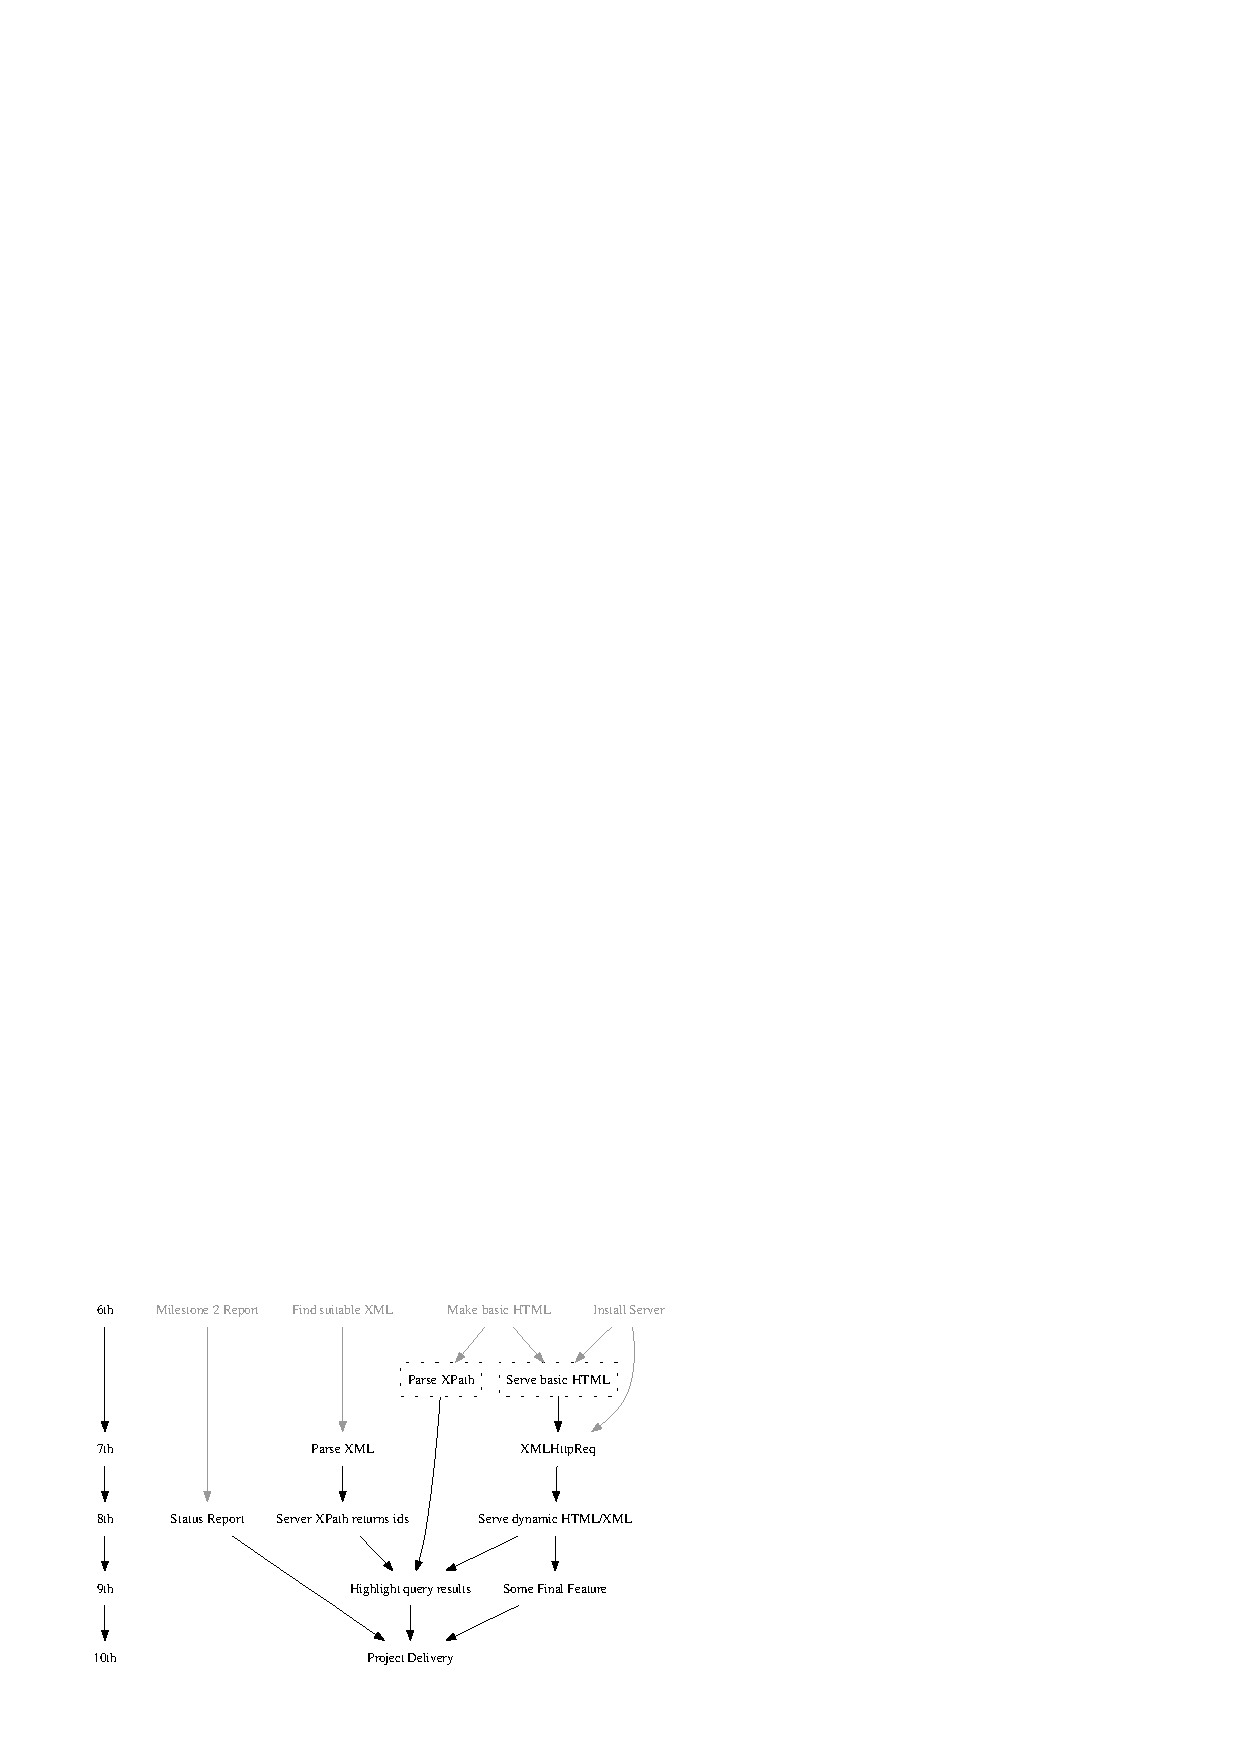
\includegraphics[width=\textwidth]{process}
\caption{Screenshot of completed project}
\end{figure}




\section{Further Work}

There are many opportunities for further work on this project, in a wide variety of areas.

Based on the strategy I plan to take with partial parsing and monadic processing, that it may be possible to have a sort of pause-return-continue loop within the processing of XPath expressions, such that, at the end of each evaluation of a subexpression, the parser pauses to return the set of nodes that have been selected, and then waits for the input of an additional subexpression- at which point it will continue parsing from the point at which it left off, without repeating any unnecessary effort. 

Additionally, the concept of streaming processing\cite{barton:streaming} would be a very interesting concept to pursue, perhaps in conjunction with the inclusion of a feature in which the user can manually specify very large documents. 

Other concepts for additional work on this project, apart from those outlined above could include any of the following:
\begin{itemize}
\item Calculating the XPath expression whose result would be a given set of nodes. This could be a corollary to the functionality provided for regular expressions at \cite{regex} 
\item Implementing the full XPath standard
\item Implementing the full XML standard
\item Determining whether a query that returns no results for a given XML document could be satisfiable given the document's DTD, as in \cite{benedikt:satisfiability}.
\item Using tree-to-table mapping with the existing range labeling to more efficiently implement various operators, such as ``//''
\end{itemize}




%%%%%%%Run spell check!%%%%%%

\nocite{xpathtokenizer}

\bibliographystyle{abbrv}
\bibliography{uno}

\end{document}